\documentclass[11pt,a4paper,twoside,titlepage]{scrbook}
\usepackage[utf8]{inputenc}
\usepackage[pdfborder={0 0 0}]{hyperref}
\usepackage{amsmath}
\usepackage{amsfonts}
\usepackage{amssymb}
\usepackage{graphicx}
\usepackage{geometry}
\usepackage{tikz}
\usepackage{amsthm}
\usepackage{algorithmic}
\usepackage{algorithm}
\usepackage{algpseudocode}
\usepackage{float}
\usepackage{cleveref}

\theoremstyle{thmstyleone}%
\newtheorem{theorem}{Theorem}[chapter]
\newtheorem{lemma}[theorem]{Lemma}
\newtheorem{corollary}[theorem]{Corollary}

\newtheorem{proposition}[theorem]{Proposition}% 

\theoremstyle{thmstyletwo}%
\newtheorem{example}[theorem]{Example}%
\newtheorem{remark}[theorem]{Remark}%
\newtheorem{observation}[theorem]{Observation}% 
\newtheorem{claim}[theorem]{Claim}% 

\theoremstyle{thmstylethree}%
\newtheorem{definition}[theorem]{Definition}%

\crefname{figure}{Figure}{Figures}

\crefname{theorem}{Theorem}{Theorems}
\crefname{lemma}{Lemma}{Lemmas}
\crefname{claim}{Claim}{Claims}
\crefname{observation}{Observation}{Observations}
\crefname{corollary}{Corollary}{Corollaries}
\crefname{section}{Section}{Sections}
\crefname{definition}{Definition}{Definitions}

\begin{document}
	
	\frontmatter

	%----- TITLE PAGE -----
	
	\begin{titlepage}
		%\noindent\makebox[\linewidth]{\rule{\paperwidth}{0.4pt}}
	
		\begin{tikzpicture}[remember picture, overlay]
		\node [anchor=north east, inner sep=0pt]  at (17.9,2)%(current page.north east)
			{
\includegraphics[height=3.5cm]{figures/tu-bs_logo.jpg}};
		\end{tikzpicture}
		
		\centering
		\vspace{4cm}
		{\scshape\huge Bachelor Thesis\par}
		\vspace{1.5cm}
		{\Huge\bfseries Computing Optimal Solutions for the Chromatic Art Gallery Problem\par}
		\vspace{2cm}
		{\huge $\ll$Jan Siemsen$\gg$\par}
		{\Large$\ll$5019321$\gg$\par}
		{\Large$\ll$Computer Science Bachelor$\gg$\par}
		
		\vfill\vfill
		Institute of Operating Systems and Computer Networks\\
		Algorithms Division
		
		\vfill
		
		\textbf{First reviewer}\par
		$\ll$Anon Anonymous, Institute of XY$\gg$\par
		\vfill
		
		\textbf{Second reviewer}\par
		$\ll$Anon Anonymous, Institute of YX$\gg$\par
		\vfill
		
		\textbf{Supervised by}\par
		$\ll$Dominik Krupke$\gg$\par
		$\ll$Phillip Keldenich$\gg$\par
		\vfill
%\begin{description}
%	\item[Supervisor]
%	\item[First Reviewer]
%	\item[Second Reviewer]
%\end{description}
		
		
		% Bottom of the page
		{\large \today\par}
	\end{titlepage}
	
	\cleardoublepage
	
	% statement of originality
	\thispagestyle{plain} % no header
	\vspace*{7cm}
	\centerline{\bfseries Statement of Originality}
	\vspace*{1em}
	\noindent
	This thesis has been performed independently with the support of my supervisor/s.
	To the best of the author's knowledge, this thesis contains no material previously
	published or written by another person except where due reference is made in the text.
	
	\par
	\bigskip\noindent Braunschweig, \today \par
	\vspace*{10mm}
	\hfill\hrulefill
	\cleardoublepage
	
	
	\chapter*{Aufgabenstellung}
	Bei der Abdeckung von Innenbereichen mit Funk- oder Infrarotsignalen ist es einerseits wichtig, dass tatsächlich jeder Bereich mit einem ausreichenden Signal versorgt ist; andererseits treten Probleme mit Interferenz zwischen den Signalen verschiedener Sender auf, solange deren Frequenzen zu ähnlich sind. Daher sollten Sender, deren Sendebereiche sich überschneiden, möglichst unterschiedliche Frequenzen verwenden (oder alternativ in jedem Bereich wenigstens ein ungestörter Sender verfügbar sein). Da das verfügbare Spektrum in der Regel nur wenige hinreichend verschiedene Frequenzen zulässt, ist es sinnvoll, die Anzahl genutzter Frequenzen zu minimieren, ohne dabei die vollständige Abdeckung aufzugeben. Die aus dieser Problemstellung resultierenden Optimierungsprobleme heißen Chromatic Art Gallery Problem oder Conflict-Free Chromatic Art Gallery Problem. \\
    In seiner Bachelorarbeit wird sich Herr Siemsen mit der Berechnung optimaler Lösungen für das Chromatic Art Gallery Problem befassen.
    Ein existierender Ansatz von Zembon et al., der sich auf den Einsatz von MIP-Solvern konzentriert, dient als Ausgangspunkt.
    Da dieser Ansatz keine frei verfügbare Implementierung aufweist, besteht Herrn Siemsens erste Aufgabe darin, diesen Ansatz zu implementieren und die Ergebnisse zu reproduzieren. \\
    Anschließend soll er alternative Lösungsansätze erforschen, wie zum Beispiel den Einsatz eines SAT-Solvers anstelle eines MIP-Solvers, was sich beim ähnlichen Dispersive Art Gallery Problem als effektiv erwiesen hat.
    Darüber hinaus können Heuristiken entwickelt werden, die als Ausgangspunkt für Lösungen dienen, und die Variante des Conflict-Free Chromatic AGP untersucht werden.
    Die Evaluation der Arbeit muss der SIGPLAN Empirical Evaluation Checklist entsprechen und einer üblichen empirischen Auswertung folgen,
    die auf einer konkreten Fragestellung, einem Experimentdesign, der Vorstellung der Ergebnisse und der Beantwortung der Fragestellung basiert.
	
	
	%---------------------
	\chapter*{Abstract}
% In this thesis, we explore optimally solving the Chromatic Art Gallery Problem on vertex guards. This problem has previously been considered by Zambon et al. using a MIP solver. We reproduce these results and propose a different approach using SAT and CP-SAT solver. The usage of SAT solvers turned out to be much better allowing to solve random simple polygons without holes of up to 30,000 vertices as well as better performance on random simple polygons with holes. Additionally, we provide a MIP and SAT formulation for a variation of the problem called the Conflict-free Chromatic Art Gallery problem. This problem has never practically been considered before and turned out to be much harder than the original Chromatic Art Gallery Problem. Still, we managed to solve random simple polygons without holes of up to 2500 vertices as well as simple polygons with holes of up to TODO vertices.
In this thesis, we explore optimally solving the Chromatic Art Gallery Problem with vertex guards. The goal is to find a set of guards that covers the entirety of a (simple) polygon whilst requiring a minimum number of colors such that each guard gets assigned a color and no two guards of the same color can have their coverage area overlapping.

Building upon previous work by Zambon et al.~\cite{zambon2014exact}, who used MIP solvers, we replicate their results and propose an alternative approach using SAT and CP-SAT solvers. Our findings show that SAT solvers outperform MIP solvers, allowing us to efficiently solve random simple polygons without holes of up to 30,000 vertices, and improve performance on random simple polygons with holes. 

Additionally, we introduce formulations for the Conflict-free Chromatic Art Gallery problem. In this variation of the problem, rather than requiring all guards covering a point to have different colors, we only ask for at least one guard to have a unique color among them. This problem has not been practically considered before and turned out to be a more challenging variation. While we make progress in solving smaller instances of this problem, further investigation is needed for larger polygon sizes.

	
	\tableofcontents
	
	%% Remove listoffigures or listoftables if not needed!
	\listoffigures
	
	\listoftables
	
	\mainmatter
	
	%!TeX root=../thesis.tex
\chapter{Introduction}
The Chromatic Art Gallery Problem (CAGP) was first introduced by Erickson and LaValle in 2010 ~\cite{erickson2010chromatic}. The problem involves finding a guard set that covers the entirety of a given polygon P, requiring the smallest number of colors to color the guards such that the visibility regions of guards with the same color do not overlap. This minimum number of colors is called the ``chromatic guard number'' $\chi_G(P)$. Another closely related problem is the Conflict-free Chromatic Art Gallery Problem (CFCAGP), where the goal is for each point in the polygon to have at least one guard with a distinct color among the guards covering that point ~\cite{bartschi2014conflict}. For both problems, finding a guard set that satisfies the constraints has been established to be NP-hard even when limiting oneself to the set of candidate guards being the vertices of the polygon ~\cite{fekete2014chromatic}~\cite{erickson2011many}~\cite{iwamoto2022vertex}. In this context, we will explore finding exact solutions using MIP, SAT, and CP-SAT solvers.

\section{Results}
Both for the Chromatic Art Gallery Problem and its conflict-free variation, we show that SAT solvers are highly efficient compared to MIP solvers. For the CAGP, they allow us to solve random simple polygons without holes of up to 30,000 vertices as well as most random simple polygons of up to 1000 vertices with 100 holes. In the case of random simple polygons without holes, they provide faster runtimes for all tested instances. In the case of random simple polygons with holes

\section{Related Work}
The complexity of the chromatic art gallery problem has been the subject of several papers covering different classes of polygons.
For a polygon with holes, it is NP-hard to decide if a fixed number $k \geq 2$ of colors is sufficient ~\cite{fekete2014complexity}. Similarly, computing the minimum number of colors needed to cover a simple polygon is NP-hard for $\Theta(n)$ colors ~\cite{fekete2014complexity}, and the same holds when limiting ourselves to arbitrary guard positions ~\cite{fekete2014chromatic}. When it comes to covering an orthogonal polygon, deciding whether a fixed number $k \geq 2$ of colors is sufficient is also NP-hard ~\cite{hoorfar2021np}.\par\noindent
However, given a polygon $P$ and a guard set $S$ of $P$, it is possible to compute an optimal coloring of $S$ so that no two members of $S$ with the same color have overlapping visibility regions in polynomial time ~\cite{erickson2011many}. For a simple polygon $P$ and a discrete set of candidate guard locations, there exists a polynomial time algorithm to compute an optimal $2$-colorable guard set considering various objectives ~\cite{fekete2014chromatic}. Additionally, for a simple polygon $P$ and a discrete set of candidate guard locations, there is an $\mathcal{O}(\log (\chi_G(P)))$-approximation algorithm that runs in polynomial time ~\cite{fekete2014chromatic}. There is also a $6$-approximation algorithm for simple orthogonal polygons with linear time and space complexity, as well as an exact algorithm for histogram polygons that runs in linear time \cite{hoorfar2021np}.\par\noindent
Since the problem remains NP-hard for most polygon classes, one might want to find lower and upper bounds on the problem.\par\noindent
In the following, we consider a few lower bounds.
For $k \geq 3$ exists a polygon $P_k$ with $4k$ vertices and $\chi_G(P_k) \geq k$ ~\cite{erickson2012art}.
For $k$ exists a polygon $P_k$ with $3k$ vertices and $\chi_G(P_k) \geq k/2$ ~\cite{bartschi2011coloring}.
For $k \geq 3$ exists a strictly monotone polygon $M_k$ with $3k^2$ vertices and $\chi_G(M_k) \geq k$ ~\cite{erickson2012art}.
For $k \geq 3$ and odd exists a monotone orthogonal polygon $R_k$ with $4k^2 + 10k + 10$ vertices and $\chi_G(R_k) \geq k$ ~\cite{erickson2012art}.
For $k$ exists a monotone orthogonal polygon $R_k$ with $4k^2$ vertices and $\chi_G(R_k) \geq k/4$ ~\cite{bartschi2011coloring}.\par\noindent
Next, we look at a few upper bounds.
For any monotone, orthogonal or general polygon $P_n$ with n vertices $\chi_G(P_n) = \mathcal{O}(n)$ ~\cite{bartschi2011coloring}.
For any spiral polygon $P_{spi}$ $\chi_G(P_{spi}) \leq 2$ ~\cite{erickson2012art}.
For any staircase polygon $P_{sta}$: $\chi_G(P_{sta}) \leq 3$ ~\cite{erickson2012art}.\par\noindent
The only paper that has addressed practically solving the chromatic art gallery problem so far is by Zambon et al.~\cite{zambon2014exact}. The paper proposes a MIP formulation of the problem and provides practical results on it. The MIP solver used in this thesis is based on the approach presented in that paper.\par\noindent
Now looking at the conflict-free chromatic art gallery problem, there has only been one paper considering its complexity so far.
For a polygon with holes, determining whether there exists a conflict-free chromatic vertex guard set with $2$ colors is NP-hard ~\cite{iwamoto2022vertex}.\par\noindent
As for lower and upper bounds, the following upper bounds were discovered.
For any monotone polygon $P_n$ with n vertices $\chi_{cfG}(P_n) = \mathcal{O}(\log n)$ ~\cite{bartschi2011coloring}.
For any orthogonal polygon $P_n$ with n vertices $\chi_{cfG}(P_n) = \mathcal{O}(\log n)$ ~\cite{bartschi2011coloring}.
For any polygon $P_n$ with n vertices $\chi_{cfG}(P_n) = \mathcal{O}((\log n)^2)$ ~\cite{bartschi2011coloring}.
As for practically solving the Conflict-free Chromatic Art Gallery Problem, there have been no publications as of date and this thesis provides a first attempt at doing so.

% \textbf{Exact algorithm for the DCAGP (Discrete Chromatic Art Gallery Problem):} \cite{zambon2014exact}
% \begin{enumerate}
%     \item Determine guard set G
%     \item Determine witness set W via placing a witness in each shadow AVP
%     \item Build Graph G$_T$ for every guard/witness a vertex and an edge whenever a guard covers a witness or two guards are conflicting
%     \item Use Upper Bound heuristic using independent sets to find a feasible K
%     \item Solve the DCAGP on G$_T$ using K:
%     \begin{enumerate}
%         \item[-] Boolean variables for K colors and for whether a color is assigned to a guard in the optimal solution
%         \item[-] minimize the number of colors used
%         \item[-] add witness covering constraints
%         \item[-] add at most one color per guard constraint (performance)
%         \item[-] add symmetry breaker constraints (performance)
%         \item[-] lazily add clique edge cover constraints (instead of edge constraints for conflicting guards)
%     \end{enumerate}
% \end{enumerate}

\section{Overview}
In the Preliminaries section, we will briefly introduce the terms used throughout this thesis. Afterward in the Theoretical Results section, we prove a few theorems that are necessary for a correct implementation of our problem formulations. In the following two sections, we provide MIP and SAT formulations for the Chromatic Art Gallery Problem and Conflict-free Chromatic Art Gallery Problem respectively. The Implementation Details section deals with the methods used to process our geometric input allowing us to convert it into MIP constraints and SAT clauses. In the Experiments section, we will benchmark our implementations on random simple polygons with and without holes. Lastly, we give a conclusion on our experimental findings and provide open problems for future research.	
	\chapter{Preliminaries}
\begin{definition}[Simple polygon]
When given a list of distinct points in the plane, the line segments between consecutive points in the list and the last and first point form the outer boundary of a simple polygon, as long as none of them cross each other. This outer boundary is a Jordan polygonal curve, and together with its interior face, it forms a simple polygon. A simple polygon with holes P, additionally contains one or more smaller simple polygons fully contained in its interior. The interior of these smaller polygons is then considered as the exterior of P.
\end{definition}

\begin{definition}[Visibility polygon]
For a simple polygon P (possibly with holes), two points p, q E P are mutually visible if the line segment between them is fully contained in P. Given a point p E P, p and all points in P visible to it form a simple polygon. We call the polygon visibility polygon of p.
\end{definition}

\begin{definition}[Guard set]
For a simple polygon P (possibly with holes), a guard set G is a set of points in P s.t. all the points in P are contained in at least one of the visibility polygons of G. We call the points of the guard set guards.
\end{definition}

\begin{definition}[Atomic visibility polygon]
When given a guard set G, we can overlay its visibility polygons to form an arrangement. We call the faces of this arrangement atomic visibility polygons. 
\end{definition}

\begin{definition}[Shadow witness set]
    
\end{definition}

\begin{definition}[2-link-visibility graph]
    
\end{definition}

\begin{definition}[Covering graph]
    
\end{definition}

\begin{definition}[Chromatic Art Gallery Problem]
    
\end{definition}

\begin{definition}[Conflict-free Chromatic Art Gallery Problem]
    
\end{definition}
	\chapter{Theoretical Shenanigans}

\begin{theorem}[Couto et al.\cite{couto2011exact}]\label{thm:shadow_coverage}
When given a polygon $P$ and a guard set $G$, a subset $G_{sub}$ of $G$ fully covers $P$ if and only if it covers all witnesses in the shadow witness set $W$ of $G$.
\end{theorem}
\begin{proof}
The necessity condition follows trivially from $W\subset P$. As for the sufficiency condition, consider the largest area $R$ that is not covered by $G_{sub}$. Because of the atomicity of AVPs, $R$ must consist of one or more AVPs. Now consider the AVP $f$ with minimal guard subset $G_{f}$ in $R$. We show that $f$ must be a shadow AVP, a contradiction. If $f = R$, then $f$ trivially must be a shadow AVP. Otherwise, consider the neighbors of $f$. For all neighbors in $R$, $G_{f}$ can not contain their guard subset as $G_{f}$ is minimal in R. As for the neighbors not in $R$, if there exists a neighbor of which the guard subset is contained in $G_{f}$, then $f$ must be covered by one of the guards in that subset and can not be part of $R$. Otherwise, $G_{f}$ does not contain any of its neighbors' guard subsets and thus is a shadow AVP.
\end{proof}

\begin{theorem}\label{thm:light_covers}
When given a polygon $P$ and a guard set $G$, the guard subsets of a light polygon form a clique in the 2-link-visibility graph $G_{vis}$ of $G$, and the cliques of all light polygons cover all edges of the graph.
\end{theorem}
\begin{proof}
The guard subset of a light polygon is formed by all the guards whose visibility polygons intersect in it, thus trivially forming a clique in $G_{vis}$. Assuming that for $g,g'\in G$ there exists an edge $(g, g')$ in $G_{vis}$ that is not covered by those cliques, then there exists an AVP $f$ that is not light and contains $g$ and $g'$ in its guard subset $G_{sub}$. As $f$ is not light there exists a neighboring AVP $f'$ whose guard subset contains $G_{sub}$. One can continue this argument with $f'$, but as the number of AVPs is finite, we will eventually reach an AVP $f^{*}$ of which the guard subset is not contained in its neighbors. Thus, $f^{*}$ is a light AVP and contains $g$ and $g'$, a contradiction.
\end{proof}

\begin{figure}[htbp]
\centering
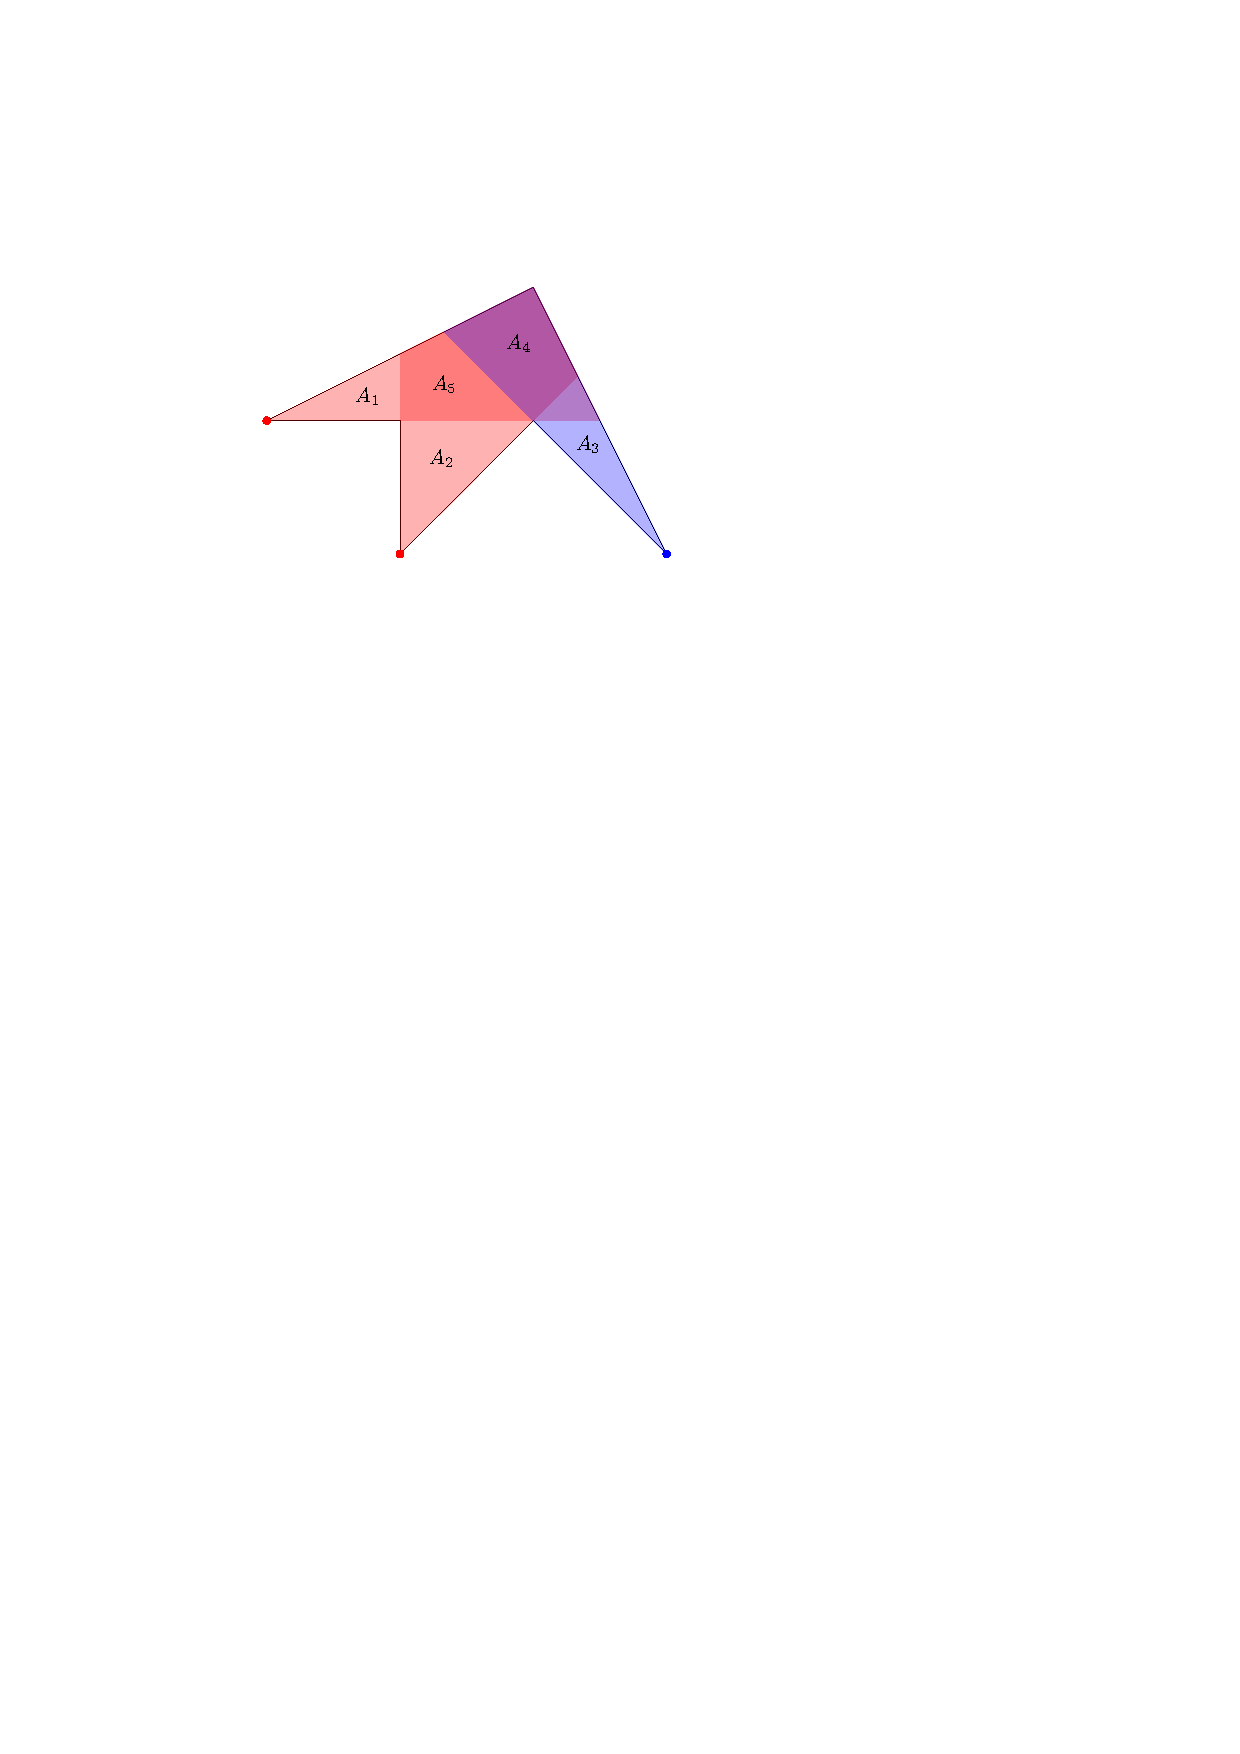
\includegraphics[scale=1.3]{Thesis/figures/conflict-free_witnesses.pdf}
\caption{Illustration for the proof of \cref{thm:conflict-free_witnesses}.}
\label{fig:conflict-free_witnesses}
\end{figure}

\begin{theorem}\label{thm:conflict-free_witnesses}
For a polygon $P$ and a guard set $G$, neither conflict-freeness of all shadow witnesses nor all light witnesses guarantees conflict-freeness within all AVPs.
\end{theorem}
\begin{proof}
To prove this theorem, we present a simple example in \cref{fig:conflict-free_witnesses}. In the figure $A_{1}$, $A_{2}$ and $A_{3}$ are shadow AVPs and $A_{4}$ is a light AVP. Each of them is covered by a guard of unique color. On the other hand, $A_{5}$ is neither shadow nor light and is covered by two guards of the same color, thus, it is not conflict-free.
\end{proof}

\chapter{Chromatic Art Gallery Problem Formulations}

In the following sections, we introduce a MIP, a SAT, and a CPSAT formulation of the Chromatic Art Gallery Problem. The MIP formulation is the one proposed by de Souza et al. \cite{zambon2014exact}, which gets modified and turned into a SAT formula for the SAT and the CPSAT formulation.

\section{MIP Formulation}

\begin{align}
\label{eq_MIP:f.0} \mbox{minimize}~& \;\sum_{k\in \{1,...,K\}} c_{k}& \\
\label{eq_MIP:f.1} \mbox{s.t. } &\sum_{g \in H}x_{gk} <= c_{k} & \forall H \in \mathcal{H}, \forall k\in \{1,...,K\}\\
\label{eq_MIP:f.2}&\sum_{g\in N(w), k\in \{1,...,K\}}x_{gk}>=1 & \forall w\in W\\
\label{eq_MIP:f.3}&\sum_{k\in \{1,...,K\}}x_{gk}<=1 & \forall g\in G\\
\label{eq_MIP:f.4}&c_{k} - c_{k+1} >= 0 & \forall k\in \{1,...,K-1\}\\
\label{eq_MIP:f.5}&\sum_{g\in G}x_{gk} - \sum_{g\in G}x_{g(k+1)} >= 0 & \forall k\in \{1,...,K-1\}\\
\label{eq_MIP:f.6}& x_{gk} \in \{0,1\} & \forall g\in G, \forall k\in \{1,...,K\}\\
\label{eq_MIP:f.7}& c_{k}\in \{0,1\} & \forall k\in \{1,...,K\}
\end{align}

The MIP formulation of the problem introduces binary variables for every guard color combination \cref{eq_MIP:f.6} and every color \cref{eq_MIP:f.7}. The guard color variables are true whenever the guard is used and is assigned the associated color in the solution. The color variables are true whenever a guard uses that color in a solution. The objective function \cref{eq_MIP:f.0} minimizes the number of colors used in the solution. The constraints in \cref{eq_MIP:f.1} are called edge clique cover constraints. They ensure that for every clique in an edge clique cover of the 2-link-visibilty-graph $G_{vis}$ and every color only one of the guards in that clique can be assigned that color. At the same time, they make sure that if a guard in that clique uses the color, the corresponding color variable must also be true. How to find an edge clique cover for $G_{vis}$, will be discussed in the Implementation Details chapter. The constraints in \cref{eq_MIP:f.2} are called witness covering constraints. They ensure that for every witness in the witness covering graph $G_{cov}$ at least one guard in its neighborhood is used in the solution, thus the witness gets covered. We call the constraints in \cref{eq_MIP:f.3} guard coloring constraints. They ensure that each guard is assigned at most one color. Technically, these constraints are not necessary to find an optimal solution, as one can simply process the solution by deciding on one color for every guard that got assigned multiple. The reason for still including these constraints is that they reduce the space of possible optimal and near-optimal solutions, which can help the solver arrive at an optimal solution faster. In the same mindset, we add the constraints \cref{eq_MIP:f.4} and \cref{eq_MIP:f.5}, which are symmetry breaker constraints. \cref{eq_MIP:f.4} ensure that when $k$ colors are used, those colors are the first k colors in $\{1,...,K\}$. As for \cref{eq_MIP:f.4}, they induce a partial order of the colors over the size of guards using that color. This reduces the possible permutations of the colors assigned to each guard in an optimal solution.

\section{SAT Formulation}

\begin{align}
\label{eq_SAT:f.0}&\lnot x_{uk} \lor \lnot x_{vk} & \forall (u,v)\in E_{G_{vis}}, \forall k\in \{1,...,K\}\\
\label{eq_SAT:f.1}&\bigvee_{g\in N(w), k\in \{1,...,K\}}x_{gk} & \forall w\in W\\
\label{eq_SAT:f.2}&\bigwedge_{1 \leq i < j \leq K} (\lnot x_{gi} \lor \lnot x_{gj}) & \forall g\in G\\
\label{eq:_SATf.3}& x_{gk} \in \{0,1\} & \forall g\in G, \forall k\in \{1,...,K\}
\end{align}

The SAT formulation of the problem differs from the MIP formulation in the way that we are not trying to minimize the number of colors used. Instead, we test whether there exists a feasible solution given a fixed number of colors K. By doing so, we can solve the SAT formula for different numbers of colors, increasing the number whenever we encounter infeasibility and decreasing it on a feasible solution, until we find the smallest number of colors for which there exists a feasible solution. The exact procedure for choosing the number of colors will be discussed in the Implementation Details chapter. Because we have a fixed number of colors, we do not require color variables like \cref{eq_MIP:f.7} anymore and restrict ourselves to the guard color variables in \cref{eq:_SATf.3}. We also omit the symmetry breaker constraints \cref{eq_MIP:f.4} and \cref{eq_MIP:f.5}, as \cref{eq_MIP:f.4} uses color variables and we found no straightforward way to model them efficiently using SAT clauses. Now for the clauses in our SAT formulation, we ensure that no two guards that share an edge in the 2-link-visibility graph $G_{vis}$ share the same color using \cref{eq_SAT:f.0}. These clauses replace the edge clique cover constraints in \cref{eq_MIP:f.1}. The reason for simply using the edges of $G_{vis}$ and not cliques is that SAT solvers are very efficient at solving large numbers of small clauses i.e. with only two variables. For the witness covering constraints \cref{eq_MIP:f.2}, we use the clauses in \cref{eq_MIP:f.1}, which have an equivalent meaning. Lastly, we use the clauses in \cref{eq_MIP:f.2} to replace the guard coloring constraints in \cref{eq_MIP:f.3}. Again, these constraints can be omitted by processing the solution at the end and we will compare the performance with and without them in the Experiments chapter below.

\section{CPSAT Formulation}

As CPSAT solvers allow for both MIP and SAT constraints, we use both the MIP and the SAT formulation and compare them against each other in the Experiments chapter.

\chapter{Conflict-free Chromatic Art Gallery Problem Formulations}

In the following sections, we introduce a MIP, a SAT, and a CPSAT formulation of the Conflict-free Chromatic Art Gallery Problem.

\section{MIP Formulation}

\begin{align}
\label{eq_MIP_cf:f.0} \mbox{minimize}~& \;\sum_{k\in \{1,...,K\}} c_{k}& \\
\label{eq_MIP_cf:f.1} \mbox{s.t. } &\sum_{g \in G}x_{gk} >= c_{k} & \forall k\in \{1,...,K\}\\
\label{eq_MIP_cf:f.2}&\sum_{g\in G}x_{gk} <= |G|\cdot  c_{k} & \forall k\in \{1,...,K\}\\
\label{eq_MIP_cf:f.3}&\sum_{g\in N(w)}x_{gk} >= u_{wk} & \forall w\in W, \forall k\in \{1,...,K\}\\
\label{eq_MIP_cf:f.4}&\sum_{g\in N(w)}x_{gk} <= 1 + |N(w)|\cdot  (1-u_{wk}) & \forall w\in W, \forall k\in \{1,...,K\}\\
\label{eq_MIP_cf:f.5}&\sum_{k\in \{1,...,K\}}u_{wk} >= 1 & \forall w\in W\\
\label{eq_MIP_cf:f.6}&\sum_{k\in \{1,...,K\}}x_{gk} <= 1 & \forall g\in G\\
\label{eq_MIP_cf:f.7}&c_{k} - c_{k+1} >= 0 & \forall k\in \{1,...,K-1\}\\
\label{eq_MIP_cf:f.8}&\sum_{g\in G}x_{gk} - \sum_{g\in G}x_{g(k+1)} >= 0 & \forall k\in \{1,...,K-1\}\\
\label{eq_MIP_cf:f.10}& u_{wk} \in \{0,1\} & \forall w\in W, \forall k\in \{1,...,K\}\\
\label{eq_MIP_cf:f.11}& x_{gk} \in \{0,1\} & \forall g\in G, \forall k\in \{1,...,K\}\\
\label{eq_MIP_cf:f.12}& c_{k}\in \{0,1\} & \forall k\in \{1,...,K\}
\end{align}

The MIP formulation for the CCAGP is similar to the one of the CAGP. We are still trying to minimize the number of colors \cref{eq_MIP_cf:f.0} and keep the same variables \cref{eq_MIP_cf:f.11} for colors and \cref{eq_MIP_cf:f.12} for guard color combinations. Additionally, we add auxiliary variables \cref{eq_MIP_cf:f.10}, called unique color witness variables, for all witness color combinations. They are true whenever there exists exactly one guard with that color in the neighborhood of that witness. To ensure that the color variables are true if and only if a guard variable of that color is true, we add the constraints in \cref{eq_MIP_cf:f.1} and \cref{eq_MIP_cf:f.2}. The constraints \cref{eq_MIP_cf:f.3} and \cref{eq_MIP_cf:f.4} ensure that if a unique color witness variable is true, exactly one guard in the neighborhood of that witness has that color. Otherwise, there can be arbitrarily many guards of that color in the neighborhood. Lastly, we keep the guard coloring constraints \cref{eq_MIP_cf:f.6} and symmetry breaker constraints \cref{eq_MIP_cf:f.7} and \cref{eq_MIP_cf:f.8} of the CAGP MIP Formulation.

\section{SAT Formulation}

\begin{align}
\label{eq_SAT_cf:f.0}&\lnot u_{wk} \lor \bigvee_{g \in N(w)}x_{gk} & \forall w \in W, \forall k\in \{1,...,K\}\\
\label{eq_SAT_cf:f.1}&\bigwedge_{(i,j)\in {G\choose 2}} (\lnot u_{wk} \lor \lnot x_{ik} \lor \lnot x_{jk}) & \forall w \in W, \forall k\in \{1,...,K\}\\
\label{eq_SAT_cf:f.2}&\bigvee_{k\in \{1,...,K\}}u_{wk} & \forall w\in W\\
\label{eq_SAT_cf:f.3}&\bigwedge_{1 \leq i < j \leq K} (\lnot x_{gi} \lor \lnot x_{gj}) & \forall g\in G\\
\label{eq_SAT_cf:f.4}& u_{wk} \in \{0,1\} & \forall w\in W, \forall k\in \{1,...,K\}\\
\label{eq_SAT_cf:f.5}& x_{gk} \in \{0,1\} & \forall g\in G, \forall k\in \{1,...,K\}
\end{align}

For the SAT formulation of the CCAGP, we test the feasibility of the SAT formula for a fixed K in the same fashion as for the CAGP, until we find a feasible solution with a minimal number of colors. We again omit the color variables and keep the unique color witness variables \cref{eq_SAT_cf:f.4} and guard color variables \cref{eq_SAT_cf:f.5}. The clauses \cref{eq_SAT_cf:f.0} are equivalent to the constraints in \cref{eq_MIP_cf:f.3}. For all witness color combinations, if the unique color witness variable of that color and that witness is true, at least one guard of the color in the neighborhood of that witness has to be true. The clauses \cref{eq_SAT_cf:f.1} are equivalent to the constraints in \cref{eq_MIP_cf:f.4}. For all witness color combinations, if the unique color witness variable of that color and that witness is true, no two guards in the neighborhood of that witness can have that color. As for \cref{eq_SAT_cf:f.2}, these clauses represent the constraints in \cref{eq_MIP_cf:f.5}. Lastly, the witness coloring constraints \cref{eq_SAT_cf:f.3} are modeled using the same clauses as in the CAGP SAT Formulation.

\section{CPSAT Formulation}
Similar to the Chromatic Art Gallery Problem, we use both the MIP and the SAT formulation for CPSAT and compare them against each other in the Experiments chapter.

\chapter{Implementation Details}

\section{Instance Processing}
The instances are given as lists of points, which represent the outer boundaries of the polygons and possible holes. First, we create a CGAL Polygon\_with\_holes\_2 using the instance input. Then, using the vertices of the polygon and its holes as the guard set $G$, we calculate the visibility regions as polygons for each guard using CGAL's "Triangular\_expansion\_visibility\_2.h" and save each guard together with its visibility polygon in a list. Afterward, we recursively overlay the visibility polygons using CGAL's "Arr\_overlay\_2.h" to obtain the AVP arrangement (\cref{alg:AVP_generation}). To be able to form the partial order over the AVPs, we overload the overlay function to save for every face a set of guards from which it was created. 

\begin{algorithm}
\caption{generate\_AVP\_recursive(guards: list[tuple[int, Polygon\_with\_holes\_2]])}\label{alg:AVP_generation}
\begin{algorithmic} 
\STATE $half\gets len(guards)/2$
\STATE $firstHalf\gets guards[:half]$ 
\STATE $secondHalf\gets guards[half:]$
\IF{$len(guards) = 1$}
    \STATE $Arrangement(guards[0][0], guards[0][1])$
\ELSE
    \STATE $generate\_AVP\_recursive(firstHalf).overlay(generate\_AVP\_recursive(secondHalf))$
\ENDIF
\end{algorithmic}
\end{algorithm}

For the CAGP, we calculate the shadow witness set. As geometric operations are expensive, instead of saving the shadow witness set as a set of points, we store each witness as an integer together with the set of guards that covers the witness as well as each guard together with the set of witnesses that the guard covers. Additionally, we store a list of the set of guards for each light AVP. For the CCAGP, we calculate the witness set as well. But because of \cref{thm:conflict-free_witnesses} just using shadow or light witnesses is not sufficient, thus we use a witness for every AVP instead. To calculate all of the above, we use \cref{alg:AVP_processing}. Afterward, we can use the light guard sets to create the visibility graph $G_{vis}$ by adding edges between guards within each set (\cref{thm:light_covers}). As for the covering graph $G_{cov}$, there is no need to create the overhead of an additional graph. Instead, we can simply check the corresponding guard set of a witness, whenever we need the neighborhood of that witness in $G_{vis}$. Lastly, we can sort the witnesses by the size of their guard sets and use the $|G|$ smallest witnesses as our initial witnesses.

\begin{algorithm}
\caption{Calculate witness sets and light guard sets}\label{alg:AVP_processing}
\begin{algorithmic}[1]
\REQUIRE $faces$ of the AVP arrangement
\STATE Initialize empty maps: $witness\_to\_guards, guard\_to\_witnesses, all\_witness\_to\_guards,\linebreak all\_guard\_to\_witnesses$
\STATE Initialize empty list: $light\_guard\_sets$
\STATE $shadow\_index\gets 0$
\STATE $all\_index\gets 0$
\FORALL{$face$ in $faces$}
    \STATE $g\_data\gets$ guard set of the $face$
    \IF{$g\_data$ is empty}
        \STATE Continue
    \ENDIF
    \STATE $is\_shadow\gets \TRUE$
    \STATE $is\_light\gets \TRUE$
    \FORALL{$half\_edge$ in $face$}
        \STATE $twin\_g\_data\gets$ guard set of the twin face of the $half\_edge$
        \IF{$twin\_g\_data$ is empty}
            \STATE Continue
        \ENDIF
        \IF{$g\_data\subset twin\_g\_data$}
            \STATE $is\_shadow\gets \FALSE$
        \ENDIF
        \IF{$twin\_g\_data\subset g\_data$}
            \STATE $is\_light\gets \FALSE$
        \ENDIF
    \ENDFOR
    \STATE $all\_witness\_to\_guards[all\_index]\gets g\_data$
    \FORALL{$g$ in $g\_data$}
        \STATE $all\_guard\_to\_witnesses[g]\gets all\_guard\_to\_witnesses[g]\cup all\_index$
    \ENDFOR
    \STATE $all\_index\gets all\_index + 1$
    \IF{$is\_shadow$}
        \STATE $witness\_to\_guards[index]\gets g\_data$
        \FORALL{$g$ in $g\_data$}
            \STATE $guard\_to\_witnesses[g]\gets guard\_to\_witnesses[g]\cup index$
        \ENDFOR
        \STATE $shadow\_index\gets shadow\_index + 1$
    \ENDIF
    \IF{$is\_light$}
        \STATE $light\_guard\_sets.append(g\_data)$
    \ENDIF
\ENDFOR
\RETURN $witness\_to\_guards, guard\_to\_witnesses, light\_guard\_sets, all\_witness\_to\_guards,\linebreak all\_guard\_to\_witnesses$
\end{algorithmic}
\end{algorithm}

\section{Initial Upper Bound}
Calculating a low initial upper bound is vital for efficiently solving the CAGP and CCAGP, as the possible number of colors K directly affects the size of the problem formulation. To achieve this, we implement the approach presented by de Souza et al. \cite{zambon2014exact}, for which K was on average only 1.7 larger than the number of colors used by the optimal solution (\cref{alg:greedy}). In the approach, we calculate weighted independent guard sets in $G_{vis}$ for as long as there are uncovered witnesses left and assign each independent guard set a different color. The weight of each guard is determined by the number of witnesses that the guard covers in the uncovered witnesses. To solve the weighted independent set formulation, we use a MIP solver.

\begin{algorithm}
\caption{Greedy Algorithm}\label{alg:greedy}
\begin{algorithmic}[1]
\REQUIRE $guard\_to\_witnesses, all\_witnesses, G_{vis}$
\STATE Initialize empty set: $solution$
\STATE $uncovered\gets all\_witnesses$
\STATE $color\gets 0$
\WHILE{$uncovered$ is not empty}
    \STATE Initialize empty list: $weights$
    \FORALL{$(guard, witnesses)$ in $guard\_to\_witnesses$}
        \STATE $weights.insert((guard, |witnesses\cap uncovered|))$
    \ENDFOR
    \STATE $solver\gets WIS\_Solver(weights, G_{vis})$
    \STATE $independent\_set\gets solver.solve()$
    \FORALL{$guard$ in $independent\_set$}
        \STATE $solution\gets solution\cup \{(guard, color)\}$
        \STATE $uncovered\gets uncovered\setminus guard\_to\_witnesses[guard]$
    \ENDFOR 
    \STATE $color\gets color + 1$
\ENDWHILE
\RETURN $color, solution$
\end{algorithmic}
\end{algorithm}

\begin{align}
\label{eq_MIP:f.0} \mbox{maximize}~& \;\sum_{(g, w)\in weights} x_{g}\cdot w& \\
\label{eq_MIP:f.1} \mbox{s.t. } &x_{u} + x_{v} <= 1 & \forall (u,v) \in E_{G_{vis}}\\
\label{eq_MIP:f.6}& x_{g} \in \{0,1\} & \forall g\in G
\end{align}

\section{Edge Clique Covers}

\begin{algorithm}
\caption{Generate Edge Clique Covers}
\begin{algorithmic}[1]
\REQUIRE $G, K$
\STATE Initialize empty lists: $matching, edge\_clique\_covers$
\STATE Initialize empty set: $covered\_vertices$
\STATE $edge\_queue\gets$ priority queue with edges from $G$ and priority negative sum of degrees of the vertices
\FOR{$i=0$ \TO $K$}
    \STATE $(u, v)\gets$ 
    \WHILE{$\{u, v\}\cap covered\_vertices$ is not empty}
        \STATE $(u, v)\gets$ pop edge with highest priority from $edge\_queue$
    \ENDWHILE
    \STATE $edge\gets (u, v)$
    \STATE $matching.append(edge)$
    \STATE $covered\_vertices\gets covered\_vertices\cup \{u, v\}$
\ENDFOR
\FORALL{$edge$ in $matching$}
    \STATE $clique\_cover\gets$ Construct Clique Cover with $G, edge$
    \STATE $edge\_clique\_covers.append(clique\_cover)$
\ENDFOR
\RETURN $edge\_clique\_covers$
\end{algorithmic}
\end{algorithm}

\begin{algorithm}
\caption{Construct Clique Cover}
\begin{algorithmic}[1]
\REQUIRE $G, edge$
\STATE $uncovered\_graph\gets G$
\STATE $clique\gets$ Build Clique with $G, edge$
\STATE $edge\_clique\_cover\gets \{clique\}$
\STATE Remove edges from $uncovered\_graph$ that are in $clique$
\STATE $edge\_queue\gets$ priority queue with edges from $G$ and priority negative sum of degrees of the vertices
\WHILE{$uncovered\_graph$ has edges}
    \STATE $edge\gets$ pop edge with highest priority from $edge\_queue$
    \STATE $clique\gets$ Build Clique with $G, edge$
    \STATE $edge\_clique\_cover\gets edge\_clique\_cover\cup {clique}$
    \STATE Remove edges from $uncovered\_graph$ that consist of vertices in $clique$
    \STATE Update priorities of edges in $edge\_queue$
\ENDWHILE
\RETURN $edge\_clique\_cover$
\end{algorithmic}
\end{algorithm}

\begin{algorithm}
\caption{Build Clique}
\begin{algorithmic}[1]
\REQUIRE $G, edge$
\STATE $(u, v)\gets edge$
\STATE $clique\gets \{u, v\}$
\STATE $candidates\gets N(u)\cup N(v)$
\WHILE{$candidates$ is not empty}
    \STATE $v\gets$ v from $candidates$ with max($\delta(v)$)
    \STATE $candidates\gets candidates\cup N(v)$
    \STATE $clique\gets clique\cup {v}$
\ENDWHILE
\RETURN clique
\end{algorithmic}
\end{algorithm}

\section{Lazy Constraints}
For the CAGP, we can restrict ourselves to the shadow witness set to check for full coverage of the polygon. But as the number of shadow witnesses can still be quite large ($O(n^2)$), we initially limit ourselves to the $|G|$ many smallest shadow witnesses within the partial order. In the case of the MIP solver, we can add possible missing witnesses early, whenever we encounter an integral feasible solution, by checking whether the corresponding witnesses of the guards of the current solution fully contain all shadow witnesses, as MIP solvers allow for the use of lazy constraints. For the SAT solver, we add possible missing witnesses, whenever we find an optimal solution for the current witness set. More on the SAT procedure can be found in the section SAT color optimization. As for the CPSAT solver, we implement both the MIP and the SAT procedure, except that CPSAT does not allow for lazy constraints. So instead, for the MIP formulation, we solve for an optimal solution, and in the case that witnesses are missing we add them and solve again. As more witnesses can only increase the optimal objective value, we can stop the search early as soon as we encounter an integral feasible solution that is equal to the previously optimal objective value.\\
For the CCAGP, according to \cref{thm:conflict-free_witnesses}, we cannot limit ourselves to either shadow or light witnesses. So instead, we have to check for all witnesses (one witness per AVP in the AVP arrangement). We will compare using the $|G|$ smallest, and largest and using all witnesses against each other. As for adding new witnesses, we proceed the same as for the CAGP, except that we cannot use lazy constraints for the MIP solver, because new witnesses add new unique color witness variables that cannot be added lazily. Thus, we use the same procedure as for the CPSAT solver.

\section{SAT color optimization}

	\chapter{Experiments}
\section{Experiment Environment}
All geometric operations were implemented using the C++ library CGAL. The visibility graph creation as well as all solvers were implemented in Python (version 3.10.14). For the MIP solvers, we used Gurobi (gurobipy version 11.0.1). The SAT solvers were implemented using PySAT (python-sat version 0.1.8.dev9). Lastly, the CP-SAT solvers were implemented with OR-tools CP-SAT solver (ortools version 9.9.3963).
The benchmarks were run in WSL2 (Windows 11, version 22H2) using an AMD Ryzen 7 7800X3D 8-Core Processor 4.20 GHz and the WSL was assigned 28 GB of RAM.

\section{SAT Solver Choice}
PySAT provides several different SAT solvers. That is why in this section, we will compare them against each other to determine, which one performs the best on our model. Additionally, we will compare using the clauses \cref{eq_SAT:f.3}(CAGP)/\cref{eq_SAT_cf:f.3}(CFCAGP) (version 1) against leaving them out and filtering the solution afterward as described in the SAT Color Optimization chapter (version 2). Due to the parameter sets becoming quite large when comparing all of the SAT solvers, we filtered out a few that performed poorly during testing beforehand. The testing was done using random simple polygons from 100 to 500 vertices and from 10 to 50 holes and each instance size had 30 polygons ~\cite{art-gallery-unicamp-page}.

\begin{figure}[htbp]
\centering
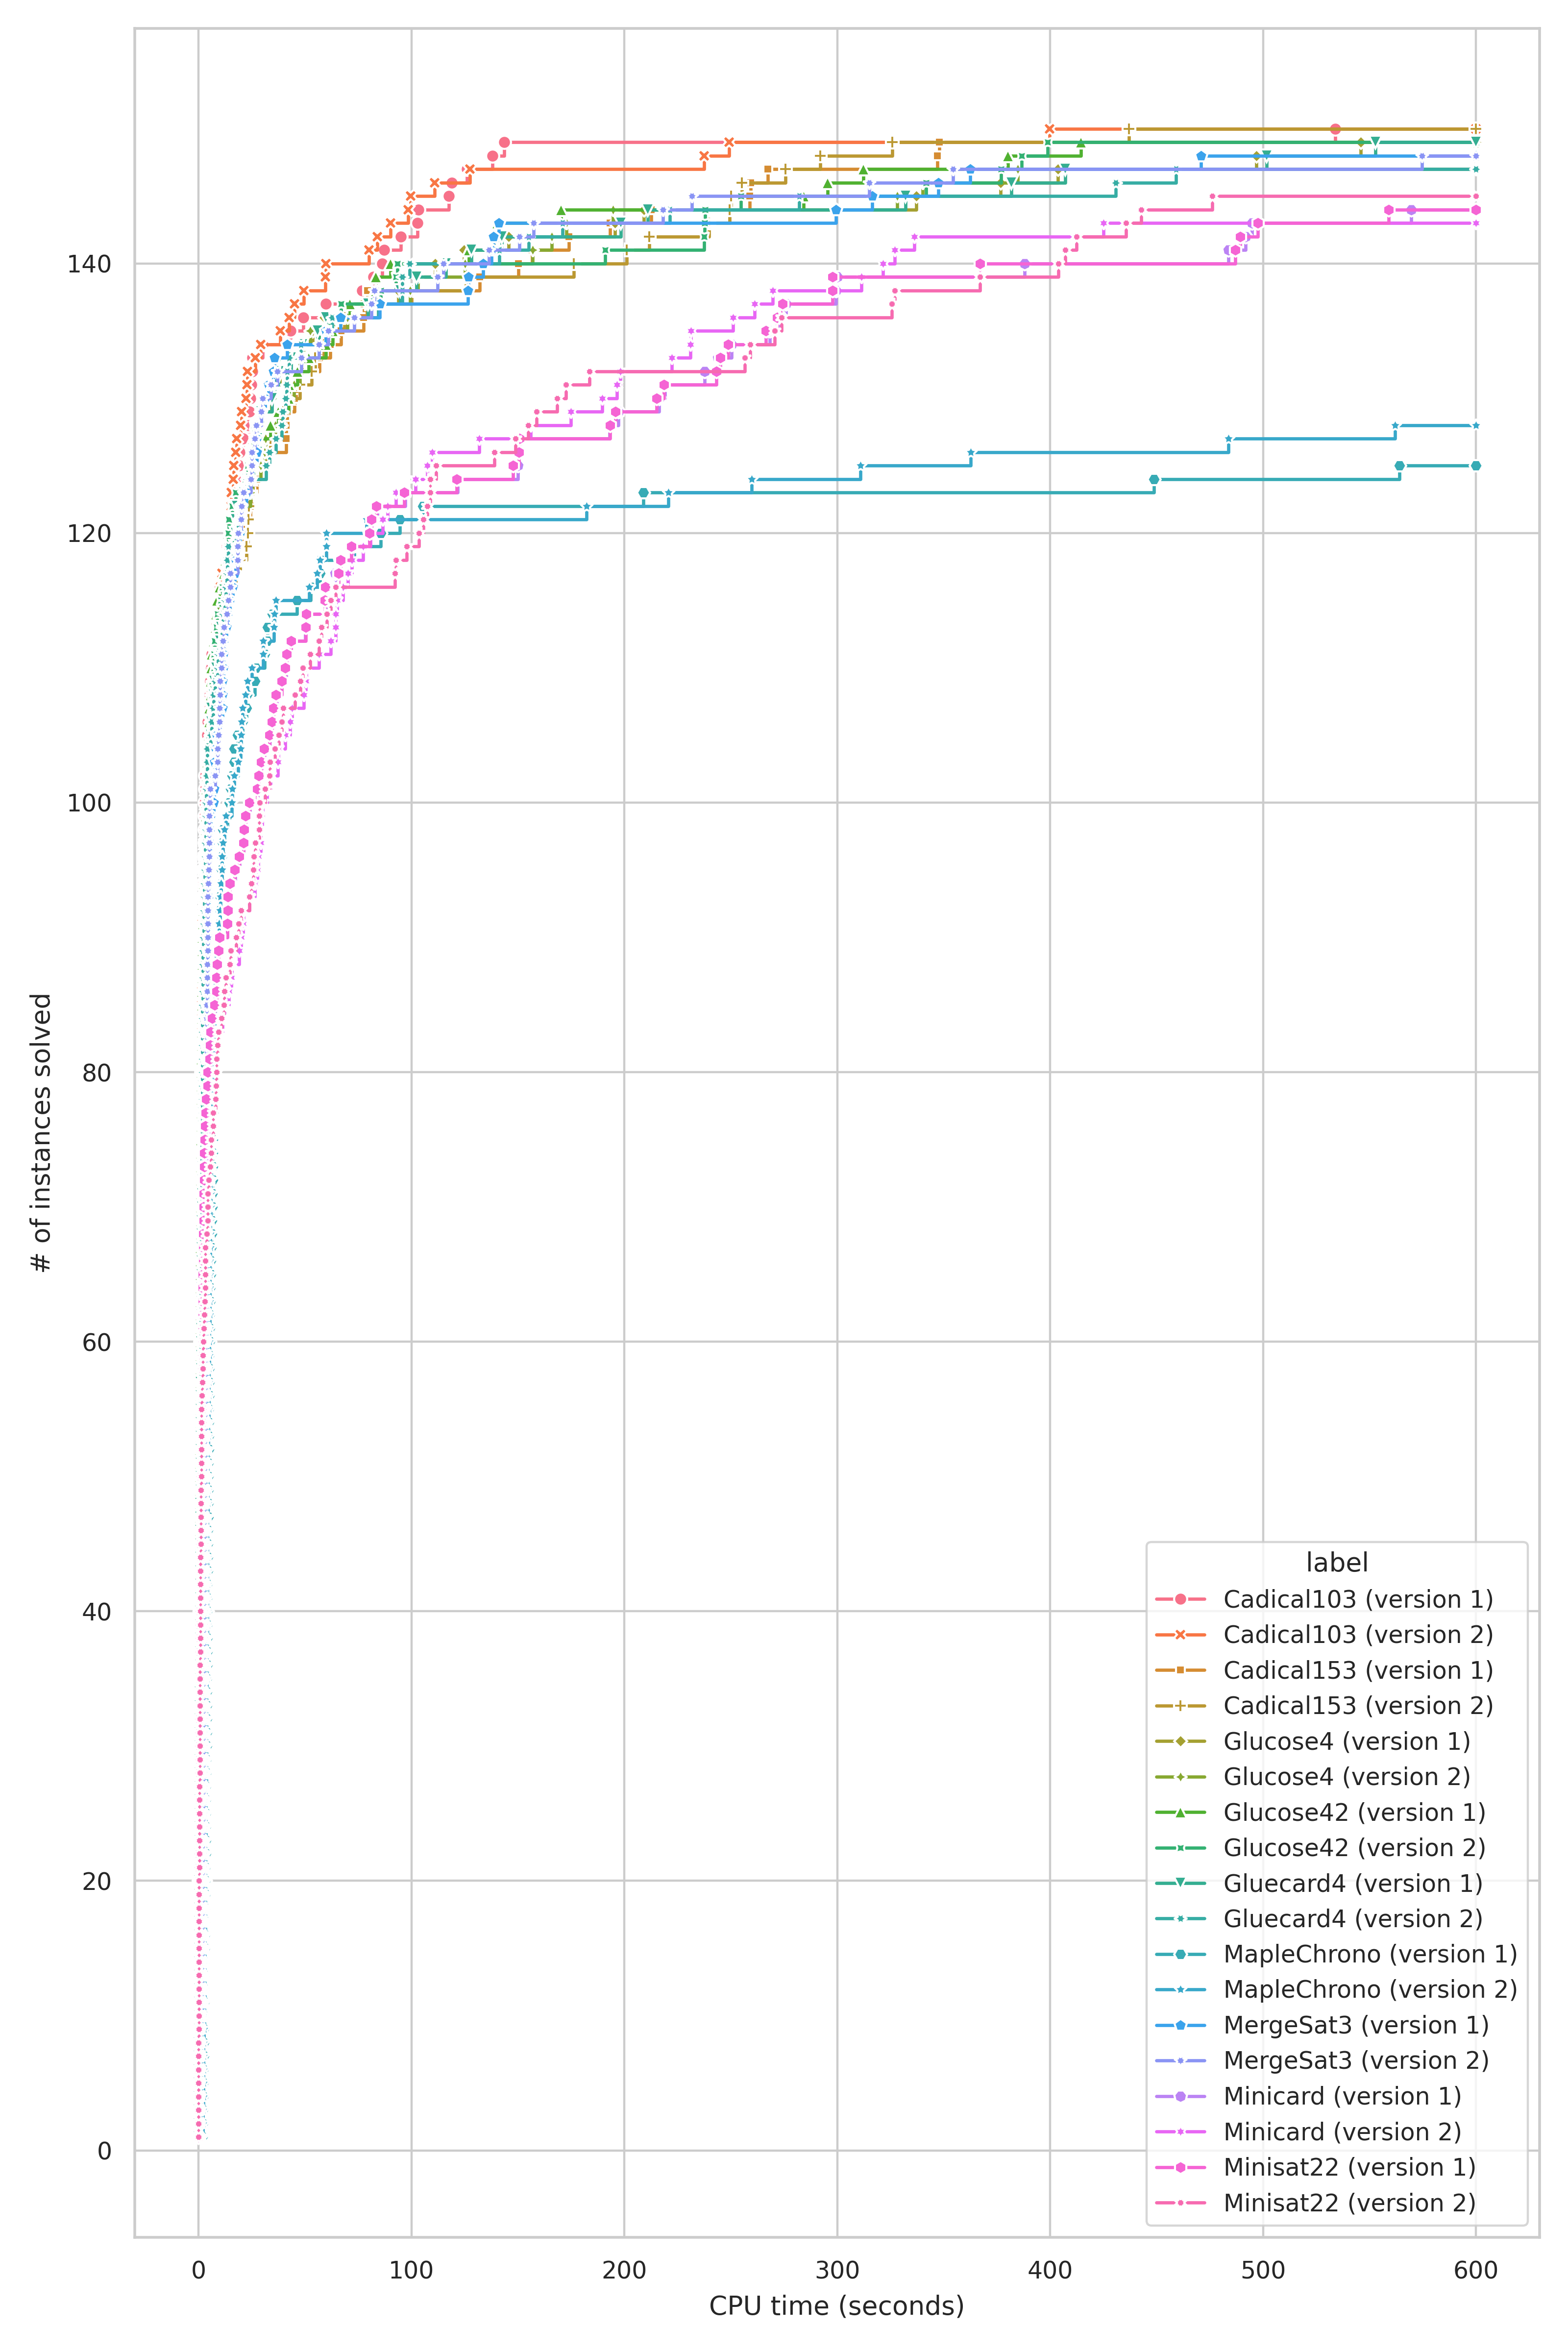
\includegraphics[scale=0.7]{Thesis/figures/minibenchmark_cactus_plot_runtime_SAT_with_holes.png}
\caption{Cactus Plot Comparing the SAT Solver Performance}
\label{fig:cactus_SAT}
\end{figure}

\begin{tabular}{llrrrrrrr}\label{tab:SAT_small_time_v1}
\toprule
 &  & Cadical103 & Cadical153 & Glucose4 & Glucose42 & MergeSat3 & Minicard & Minisat22 \\
vertices & holes &  &  &  &  &  &  &  \\
\midrule
100 & 10 & 4 & 0 & 1 & 3 & 0 & 2 & 1 \\
\cline{1-9}
200 & 20 & 2 & 2 & 4 & 6 & 0 & 1 & 1 \\
\cline{1-9}
300 & 30 & 7 & 3 & 0 & 2 & 1 & 1 & 0 \\
\cline{1-9}
400 & 40 & 5 & 1 & 3 & 6 & 0 & 0 & 0 \\
\cline{1-9}
500 & 50 & 4 & 0 & 1 & 3 & 0 & 2 & 0 \\
\cline{1-9}
\bottomrule
\caption{Number instances with lowest runtime for version1 solvers}
\end{tabular}

\begin{tabular}{llrrrrrrrrr}\label{tab:SAT_small_time_v2}
\toprule
 & & Cadical103 & Cadical153 & Glucose4 & Glucose42 & Gluecard4 & MapleChrono & MergeSat3 & Minicard & Minisat22 \\
vertices & holes &  &  &  &  &  &  &  &  &  \\
\midrule
100 & 10 & 3 & 2 & 0 & 4 & 2 & 0 & 0 & 3 & 5 \\
\cline{1-11}
200 & 20 & 6 & 1 & 1 & 2 & 2 & 0 & 1 & 0 & 1 \\
\cline{1-11}
300 & 30 & 9 & 2 & 1 & 2 & 1 & 0 & 0 & 0 & 1 \\
\cline{1-11}
400 & 40 & 3 & 3 & 1 & 3 & 4 & 0 & 0 & 1 & 0 \\
\cline{1-11}
500 & 50 & 10 & 0 & 1 & 4 & 1 & 2 & 1 & 0 & 1 \\
\cline{1-11}
\bottomrule
\caption{Number instances with lowest runtime for version2 solvers}
\end{tabular}

\section{CP-SAT Formulation Comparison}
In this section, we will compare using the MIP formulation against the SAT formulation with and without the clauses \cref{eq:_SAT:f.3}(CAGP)/\cref{eq_SAT_cf:f.3}(CFCAGP) for the CP-SAT solver. 

\section{MIP Parameter Set}
Gurobi allows us to set various parameters, which can help improve the runtime of the solver depending on the model. During testing, we used the model.tune() function on a few handpicked instances to determine a good parameter set. Note that setting the parameters drastically improves the runtime of the solver and one might want to further improve them in the future. In the following, we will list the parameters used for the CAGP MIP solver:
\begin{itemize}
  \item 
  \item 
  \item 
\end{itemize}
In the following, we will list the parameters used for the CFCAGP MIP solver:
\begin{itemize}
  \item 
  \item 
  \item 
\end{itemize}

\section{MIP vs. SAT vs. CP-SAT}
In this section, we will compare the performance of the MIP, SAT, and CP-SAT solver against each other on various polygon types.

\subsection{Simple Polygons}

\subsection{Orthogonal Polygons}

\subsection{Simple Polygons with Holes}

\subsection{Random von Koch Polygons}

	\chapter{Conclusion (and Future Work)}

In conclusion, this thesis addressed optimally solving the Chromatic Art Gallery Problem (CAGP) and its conflict-free variant (CFCAGP) by employing SAT formulations and color optimization strategies, alongside the implementation of Mixed Integer Programming (MIP) and Constraint Programming (CP-SAT) techniques. Extensive testing on random simple polygons with and without holes demonstrated the superiority of SAT solvers over MIP solvers, particularly on polygons without holes. Specifically, SAT solvers enabled the solution of random simple polygons without holes of up to 30,000 vertices for CAGP and improved performance on instances with holes, allowing to solve most instances of up to 1000 vertices and up to 100 holes.

Moving forward, there are several avenues for further research and improvement. Firstly, finding better heuristic methods for CFCAGP to achieve lower initial bounds could lead to better performances, especially for larger instances. Additionally, investigating the existence of a small atomic visibility polygon subset to use as a witness set that guarantees conflict-freeness, or proving its non-existence, could provide valuable insights into the problem's inherent complexity.

% -designed SAT formulation and color optimization scheme
% -implemented MIP, SAT, and CP-SAT for CAGP
% -designed MIP and SAT formulation for CFCAGP
% -implemented MIP and SAT for CFCAGP

% -did tests on random simple polygons with and without holes
% -SAT turned out to be much better on simple polygons without holes as well as better on with holes

% Future Work:
% -find a better Heuristic for CFCAGP for lower Initial Bound
% -try to find a small AVP subset that guarantees conflict-freeness or prove that no such set exists
% -potentially improve MIP or SAT formulation for the CFCAGP

% This is the end of your thesis! 
% Give a summary of what you did.

% You can also write down possible future work you or other people could look at.
	
	\bibliographystyle{abbrv}
	\bibliography{bibliography.bib}

\end{document}